\chapter*{Appendix/付録} % 章番号を出さない
\addcontentsline{toc}{chapter}{Appendix/付録} % 目次に載せる

%Appendix/付録.

% 付録は chapter の 1 つとして作りますが、章番号は表示しません。
% また付録の 1 つずつはアルファベットで番号付けをするのが一般的です。
\setcounter{section}{0} % section の番号をゼロにリセットする
\renewcommand{\thesection}{\Alph{section}} % 数字ではなくアルファベットで数える
\setcounter{equation}{0} % 式番号を A.1 のようにする
\renewcommand{\theequation}{\Alph{section}.\arabic{equation}}
\setcounter{figure}{0} % 図番号
\renewcommand{\thefigure}{\Alph{section}.\arabic{figure}}
\setcounter{table}{0} % 表番号
\renewcommand{\thetable}{\Alph{section}.\arabic{table}}

\begin{figure} % 特に強い理由がない限り、[htbp]のような指定はしないでください。
  \centering
  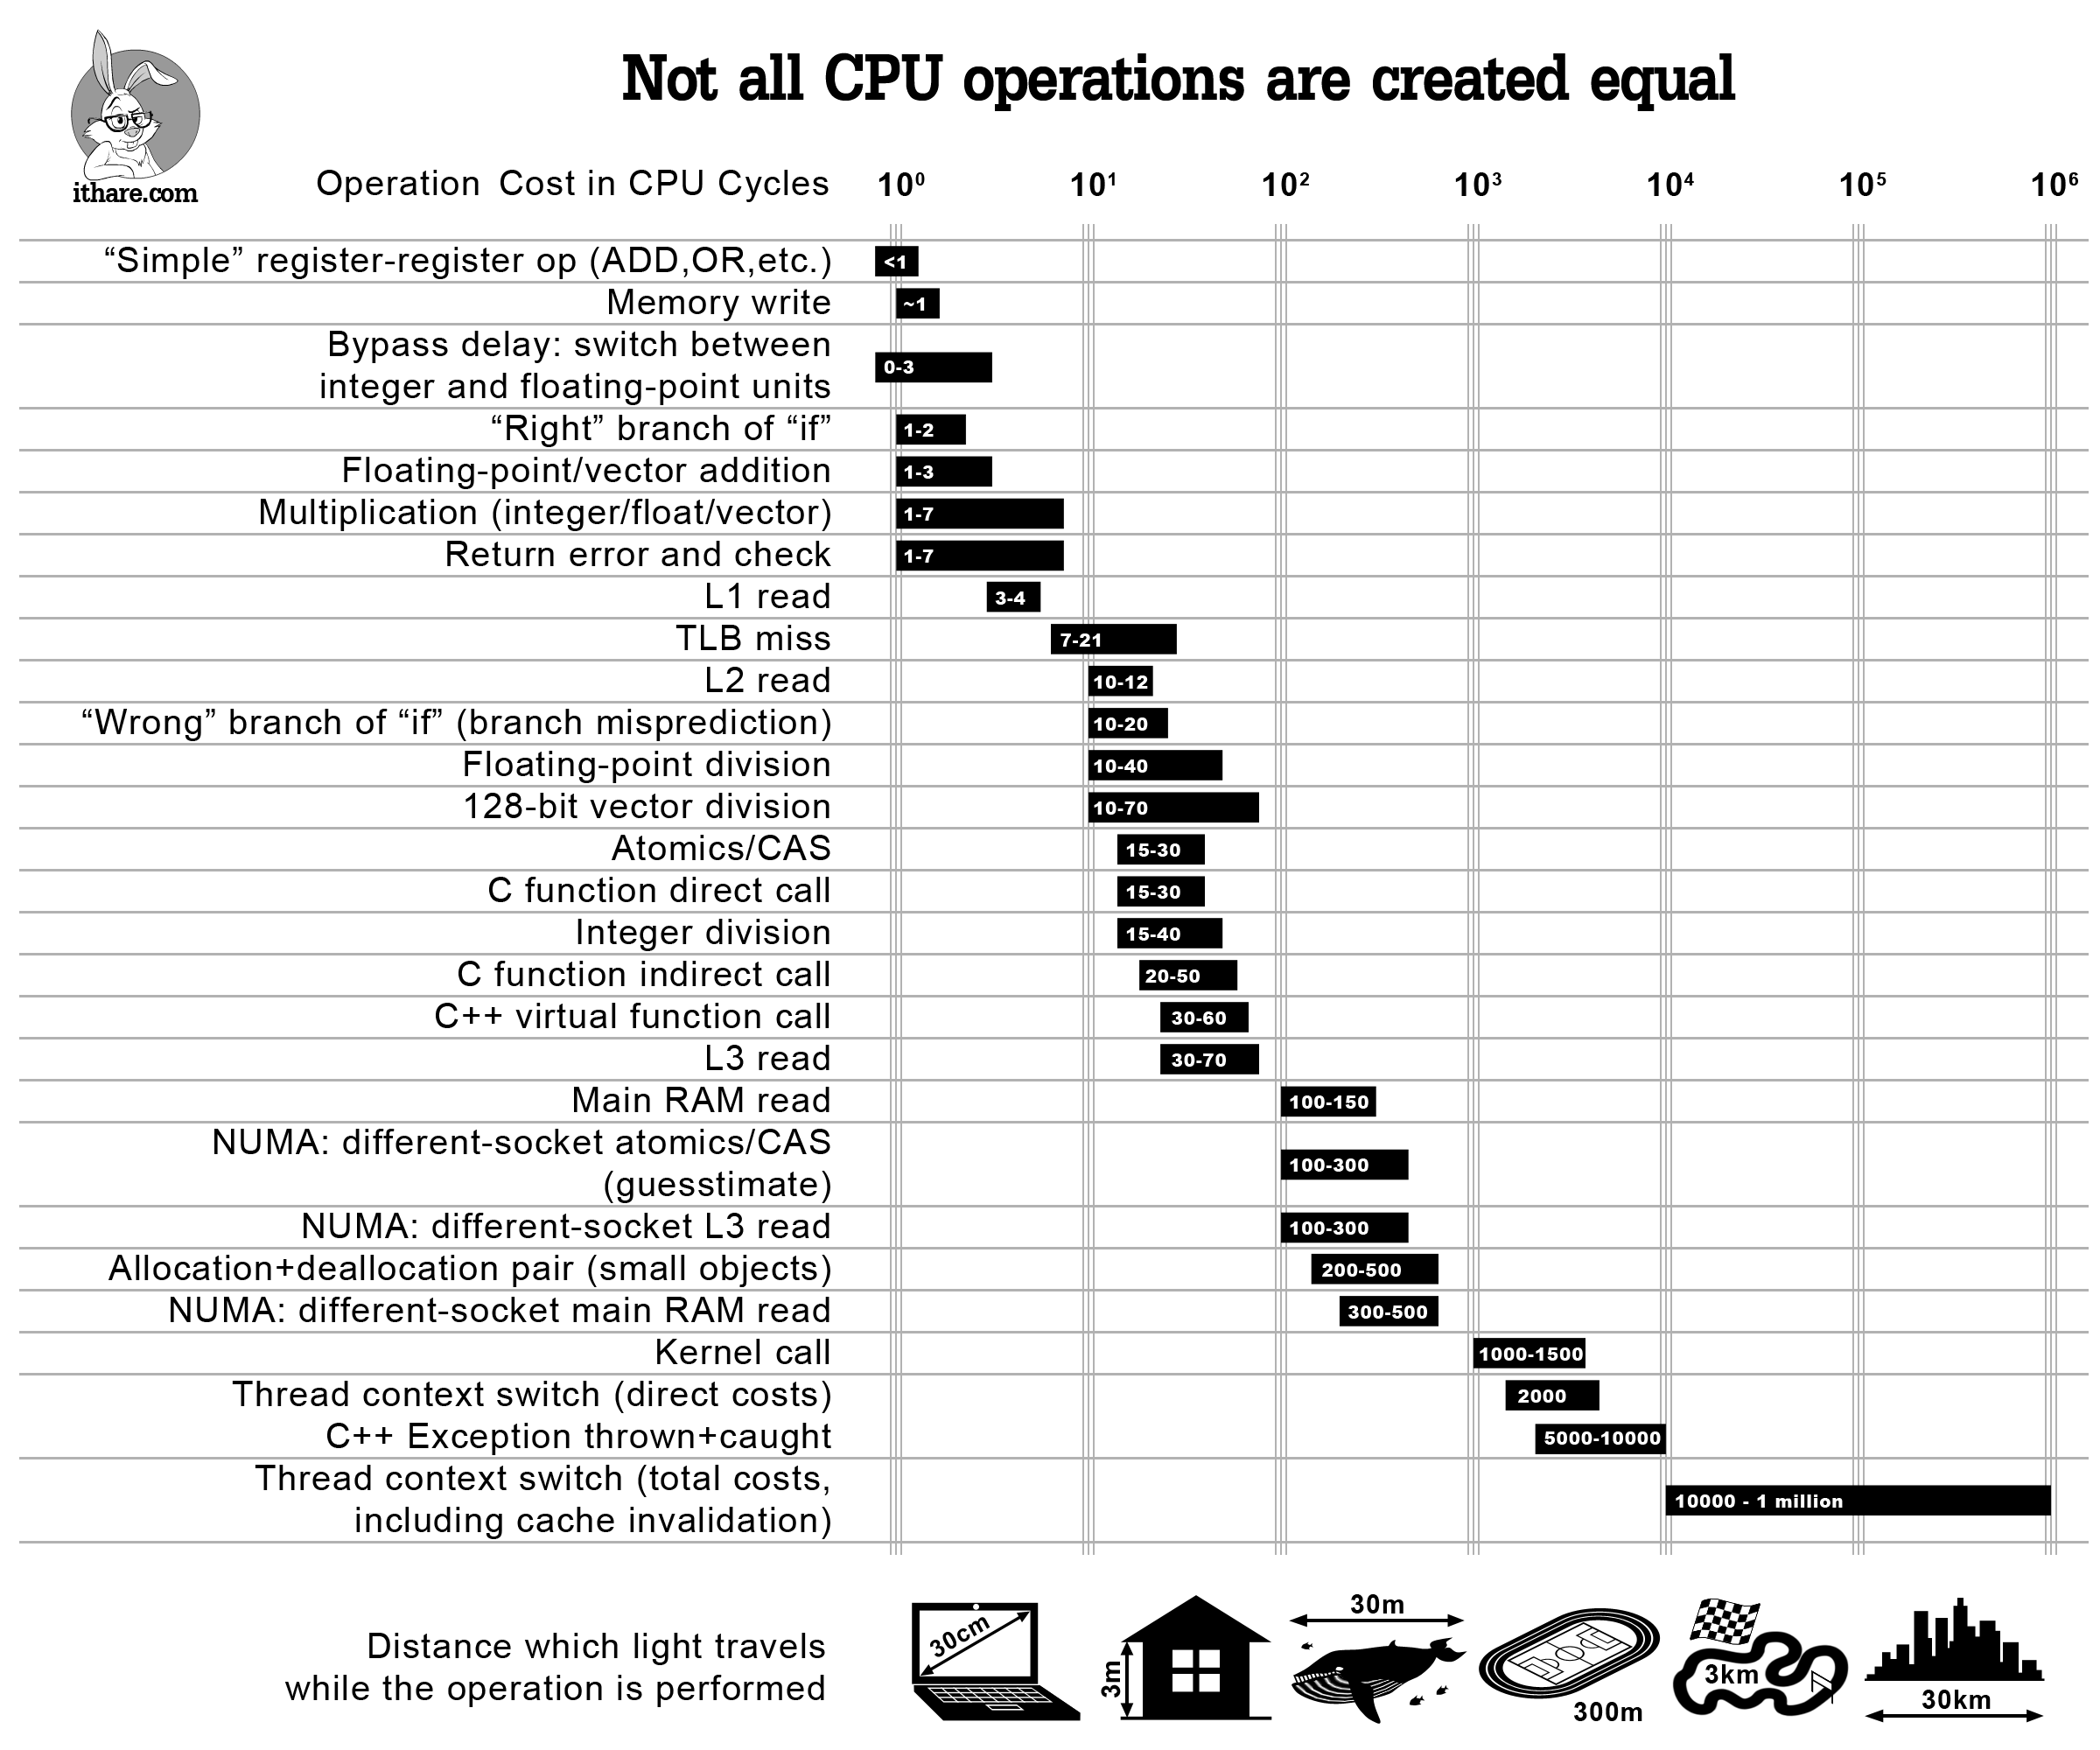
\includegraphics[width=17.25cm]{./fig/part101_infographics_v08.png}
  \caption{
    Infographics: Operation Costs in CPU Clock Cycles \citep{NoBugsHare2016}.
  }
  \label{fig_part101_infographics}
\end{figure}

%\section{セクション1}
%内容.

%\section{セクション2}
%図/表など.

